
%(BEGIN_QUESTION)
% Copyright 2013, Tony R. Kuphaldt, released under the Creative Commons Attribution License (v 1.0)
% This means you may do almost anything with this work of mine, so long as you give me proper credit

Examine this process trend showing the PV, SP, and Output of a loop controller:

$$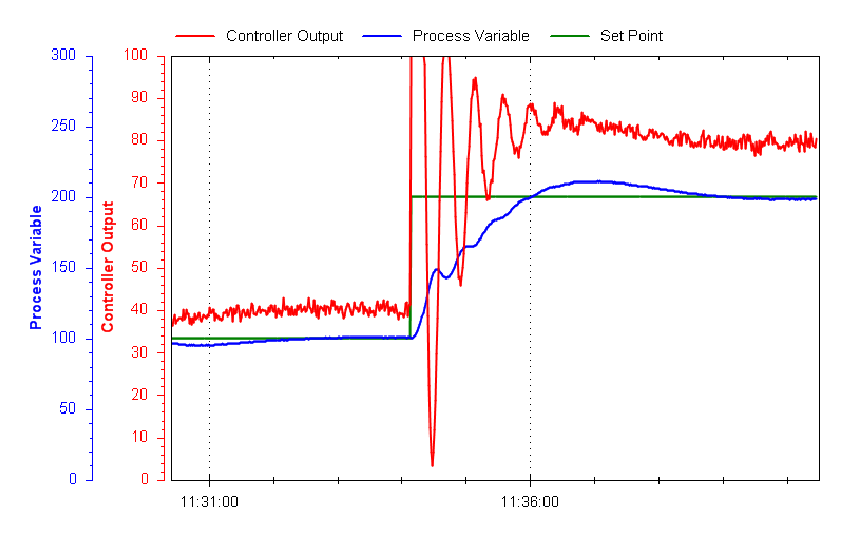
\includegraphics[width=15.5cm]{i02637x01.eps}$$

Based on what you see here, determine the following:

\begin{itemize}
\item{} Whether this is an open-loop or a closed-loop response
\item{} Whether the controller is (or needs to be) {\it direct-acting} or {\it reverse-acting}
\item{} If possible, identify any problems with the field instrumentation
\item{} If possible, identify any problems with the controller PID tuning
\item{} Qualitatively identify the kind of PID tuning we will need for robust control
\end{itemize}

\underbar{file i02637}
%(END_QUESTION)





%(BEGIN_ANSWER)

This is a {\it closed-loop test}, based on the fact the output signal responds dynamically to the changing process variable, as well as to the step-change in setpoint.

\vskip 10pt

This is a {\it reverse-acting} controller: the output steps up when the setpoint steps up (implying the output would step down if the process variable stepped up).

\vskip 10pt

There do not appear to be any field instrumentation problems revealed in this trend.  A manual-mode (open-loop) test would be more informative in that regard, but it appears as though the process is very quick to respond with little dead time or other lags.

\vskip 10pt
  
The controller tuning is clearly too aggressive for this process.  Note the ``porpoising'' action of the PV as it approaches SP following the SP step-change.  Only two types of controller action can cause this to occur: {\it proportional}, or {\it derivative}.  Porpoising is when an oscillation occurs in the PV prior to it crossing setpoint, which explains why integral action cannot ever be to blame for porpoising: the only way a loop oscillation can occur is when the final control element oscillates as well (i.e. changes direction), and since integral action will never change direction until PV crosses SP, oscillations that occur on one side of SP cannot be caused by integral action.  Looking at the phase shift between PV and output during the oscillations, it appears the output peaks may slightly lead the PV peaks, but only slightly.  This suggests that proportional is the action that is too aggressive (if it were derivative, there would be more of a leading phase shift).

\vskip 10pt

This is definitely a self-regulating process, as revealed by the fact a new output value is required to achieve a new setpoint value.  This means integral control action will definitely be necessary.  Good control will require less gain and perhaps a bit more derivative action to help cancel the lag.  Integral action looks just fine where it is right now, with just a little SP overshoot.

%(END_ANSWER)





%(BEGIN_NOTES)


%INDEX% Process troubleshooting: diagnosing problem via trend recording

%(END_NOTES)


